\setlength{\footskip}{8mm}

\chapter{METHODOLOGY}
\label{ch:methodology}

\textit{Court cases can be structured as legal arguments between the plantiffs, defendants and the Court. The arguments that stand in the end can be said to be the winning argument.
In this study we will:  1.) choose legal disputes related to marine insurance where the issue is with proximate cause  2.) identify the rules, facts and arguments in the case, and structure the case to fit into the Argumentation Framework. 3.) Structure the case to fit into the Argumentation Framework. 4.) Evalute the arguments in PROLOG.}

\section{Flota Mercante Dominicana v American Manufactureres Mutual Insurance Company}
% FACTS -----------------------------------------------------------------------------------

\newcommand{\factOne}{Plaintiff was the owner of the SS SANTO DOMINGO which burned and sank in the harbor of Santo Domingo, Dominican Republic, following shelling by members of the U.S. Armed Forces on May 4 and 5, 1965.}

\newcommand{\factTwo}{On April 24, 1965, the vessel cleared New York bound for Santo Domingo. The same day the news of the uprising in the Dominican Republic reached the ship}

\newcommand{\factThree}{According to the testimony of the ship’s captain, the broadcasts were greeted with nervous excitement by the crew. There was considerable drinking of alcoholic beverages, much hanging about the radio operator’s quarters and a general loosening of the crew’s discipline. A couple of days out of Santo Domingo, a deputation led by the first cook waited on the captain and persuaded him to permit transmission of a message sympathetic to the new constitution.}

\newcommand{\factFour}{On approaching the harbor of Santo Domingo, the captain held a meeting of the officers to discuss the question of putting into the harbor. The captain’s orders on leaving New York were to proceed to Santo Domingo, and he had received no change in those orders. He had had previous experience with navigating during revolutions, coups and uprisings in the Dominican Republic, none of which had resulted in seriously damaging consequences. Moreover, the atmosphere on ship was tense (the captain slept with a hand gun beneath his pillow), and the crew had made it clear by their behavior that they wished to enter Santo Domingo. In these circumstances, it was decided to enter the port.}

\newcommand{\factFive}{The ship went into Santo Domingo on April 29 and tied up in the Ozama River about 200 meters from a fort then in the hands of National Police loyal to the regime which had been in power when the troubles broke out. The captain gave both crew and passengers instructions to remain on the ship while he went ashore to investigate the situation. The captain attempted to get in touch with the owners of the vessel and to ascertain the conditions in the town. He quickly discovered that he was in the center of a battlefield and he was unable to return to the ship. }

\newcommand{\factSix}{It is unclear what the crew and passengers did to care for themselves, but the succeeding events suggest that within the next several hours each sought safety or excitement with the army of his choice. }

\newcommand{\factSeven}{The next day the forces in the fort next to the ship, roughly 1,000 National Police, came under heavy pressure from the new constitutionalists, who appear to have taken command of those parts of the city lying on the side of the fort away from the river. Further, the National Police in the fort had had nothing to eat for three days. An evacuation of the fort was ordered. Four to five hundred of the retreating police went aboard the SS SANTO DOMINGO, which apparently was empty at that time, seeking refuge, food and modes of escape from the opposing forces. An unsuccessful attempt was made to release the ship from her moorings (by firing machine gun volleys at the cables), a couple of the lifeboats were used to ferry the troops across the Ozama River and whatever food and clothes were found aboard were taken. Within the space of several hours, the ship was abandoned by the retreating police forces.}

\newcommand{\factEight}{The vessel was then rapidly occupied by the rebel forces. The new occupants of the ship used it to direct fire at elements of the 82nd Airborne Division which had been sent to the Dominican Republic under the executive order of President Johnson to protect American nationals and had taken up positions on the other side of the Ozama River. There were exchanges between the American and Dominican rebel forces which came to an end when the Americans resorted to the use of 106 mm explosive shells. Hits by two of these shells on May 4th and 5th caused the ship to burn and sink so that she became a constructive total loss.}
%\FACTS -----------------------------------------------------------------------------------

\subsection{Introduction}

The dispute follows a sequence of events that led to the sinking of the ship SS SANTO DOMINGO during an uprising in Dominican Republic.
The main issues that led to the dispute are disagreement on the proximate cause and ambiguity in in insurance contract.

% TODO: What is task of the ship?

\subsubsection{The Insurance Policies}

The insurance policies define the circumstances and exemptions under which the insured can make a claim to the insurer for a loss. If the loss falls under these valid circumstances, the insurer must pay the insured for the loss.

\textbf{The War Risk Policy}

The war risk policy protects the insured from losses that occur due to the risks of war.

It contains 2 exemptions that are relevant to this case.

1. If loss is due to capture, seizure, arrest, restraint, detainment, preemption, confiscation or requisition by the country in which the vessel is owned or registered is not covered.

2. If loss occurs after requisition by the country in which the vessel is owned or registered, it is not covered.

\textbf{The Hull Policy}

The hull policy protects the insured from loss that occurs due to damage to the ship.

One type of loss that could occur which is covered by this policy relevant to the case is loss due to barratery by master and crew.

The policy also contains one exemption relevant to this case: The free of capture and seizure clause, which effectively removes the war risk coverage from the hull policy.  

\subsubsection{Finding the proximate cause}

To find out who is liable, the Court has to find the proximate cause of the loss and then decide if the cause falls under the exceptions of the policy.

To achieve a degree of certainty in finding liability,
courts have relied on the maxim of \textit{causa próxima non remota spectatur}  \cite{marineInsuranceAct55}.

Therefore by looking backwards from the events that have caused loss, courts find the first cause from which the event flows in a natural, inevitable manner which could be called the "real efficient cause of the loss".

The courts must use common sense in deciding which strand in the net of causation is the proximate cause of the accident.

\subsubsection{Resolving ambiguous terms in the policy}

Courts follow the \textit{contra proferentem canon} to resolve ambiguous terms in a contract. According to this, the court should construe the ambiguities of a contract against the writer of the contract. 

\subsubsection{Events that led to the loss}

E1: SS SANTO DOMINGO set sail from New York to Santo Domingo, The same day as news of an uprising there.

E2: News of rebellion led to considerable drinking and loosening of the crew's discipline. 

E3: A deputation led by the first cook waited on the captain and persuaded him to permit transmission of a message sympathetic to the new constitution

E4: On approaching the harbor, the captain held a meeting of the officers to discuss the question of putting into the harbor, where it was decided to enter the port.

E5: The ship was docked 200 meters from a fort held by the National Police (loyal to the regime).

E6: The captain left the ship to investigate the situation, ordering the crew and passengers to remain on the ship. The captain soon discovered he was in the middle of a battlefield and was unable to return to the ship. 

E7: Within several hours the crew and passengers deserted the ship.

E8: National Police (numbering ~1000) occupying up in the fort were ordered to evacuate it.  

E9: 400-500 of the retreating police went aboard the empty ship seeking refuge, supplies and modes of escape from the opposing forces. After unsuccessfully attempting to release the ship from it's moorings, the police abandoned the ship with whatever food and supplies that were found along with some lifeboats.

E10: The vessel was soon occupied by rebel forces, who used it to direct fire at American forces. In the resulting exchange of fire, the ship was sunk, resulting in it's total constructive loss.

% \begin{figure}[H]
%   \centering
%   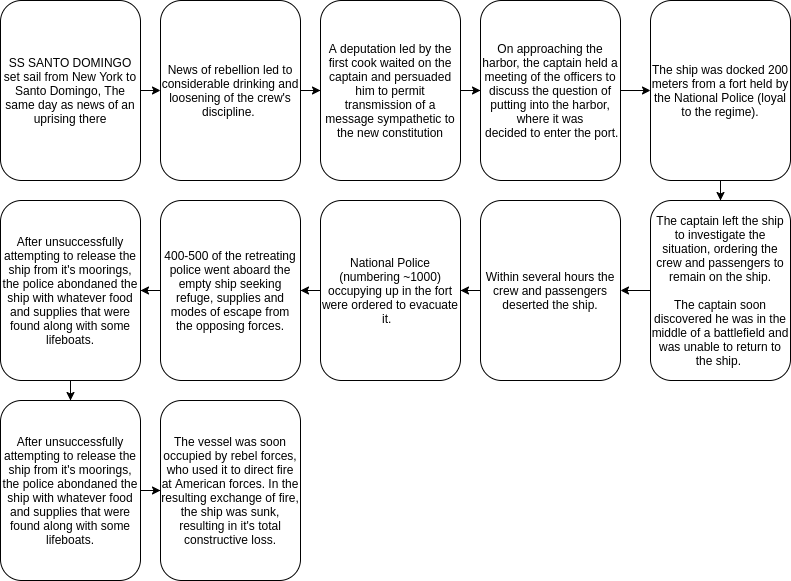
\includegraphics[width=5in]{figures/story.png}https://www.overleaf.com/project/5eb80d515c4db400012d0f3e
%   \caption[Timeline of events]{\small timeline of the events that led to the sinking of the ship.}
%   \label{fig:story}
% \end{figure}

\subsubsection{First Claim - Under the War Risk Policy}

    The ship owner makes a claim under War Risk Policy for the loss occurred in event \textit{E10}.
    
    The defendant makes two arguments about the proximate cause here, claiming these causes are not covered by the war risk policy:
    
    1. The first argues that the proximate cause falls under barratry by the crew, which is not covered by the war risk policy (at events \textit{E2, E3, E4, E5, E6, E7}), but by the hull policy.
    
    2. The second argues that loss was due to \textit{captive, seizure, arrest, restraint, detainment, preemption, confiscation or requisition} by the Dominican government in event \textit{E9}, which is also not covered by the war risk policy.
    
    Following the maxim of \textit{causa próxima non remota spectatur}, the Court determined that the barratry of the master and crew (if it existed) nor the actions of the Dominican government forced the actions of the rebel or American forces to start firing at each other. Therefore the sinking of the ship is proximately caused by risks of war.
    
    The defendant makes one more argument, arguing that irrespective of the proximate cause of loss, the ship was requisitioned (at \textit{E9}) before loss occurred (at \textit{E10}), which cancels the war risk insurance.
            
    The Court found that the term \textit{requisition} to be ambiguous. The term \textit{requisition} is not defined properly by either party, therefore the contract is read in a manner which construes the ambiguities against the party which wrote the contract (i.e. the defendant, AMMI). 
    
    Two sources the court looked at to define requisition:
    
    1. Oppenheim describes requisition as "the name for the demand for the supply of all kinds of articles necessary for an army." 2 Oppenheim's International Law (7th ed., Lauterpacht, 1955) § 147
    
    2. Article LII of the Second Hague Conventions signed by both the U.S. and the Dominican Republic lays out rules for the making of requisitions: that they shall be made only by the commander in the locality and shall be paid for as far as possible in cash or a receipt given. Although, this article covers land warfare, and the particular article deals with authority over the territory of a hostile state. Nevertheless, both these sources suggest that in requisitioning there is an aspect of formalism which flows from considered military decisions. That element is not present in the retreat of the National Police across the decks of the SS SANTO DOMINGO.
     
     Another way to come to the definition of requisition, is by looking at the context from the policy:
     
     \textit{ "...any claim arising from capture, seizure, arrest, restraint, detainment, preemption, confiscation or requisition"...}
     
     It is reasonable to assume that this list is more than repetition and that something more is meant by requisition than was meant by the seven preceding words. That is re-enforced when requisition alone is singled out as a basis for automatic termination.
     
     This special treatment of requisition separate from the usual incidents of war risk again points toward the process of formal demand and taking that was indicated by Oppenheim and the Second Hague Conventions. Such an interpretation also seems to make business sense, being aimed at ending the liability of the war risk underwriter when the ship is formally taken by a government against whom the owner would have a claim for payment and whose use of the ship might well entail risks uncalculated by the underwriter when the policy was issued.
     
     \textit{Requisition} is thus interpreted as a more formal civil condemnation, which does not exist in this case. The policemen simply rummaged through the goods and took the lifeboats with no due process, and therefore there is no requisition. Thus, the loss falls under the war risk policy.
     
\subsection{Rules}

\subsubsection{War Risk Policy} 

    \textbf{If:} loss is due to:
    
    \begin{enumerate}
         \item the risks of hostilities or warlike operations including damages suffered from "weapons of war"
    \end{enumerate}
    
    
    \textbf{Then:} The loss is covered by the war risk policy.
        
\subsubsection{War Risk Policy - Exemption 1}

    \textbf{If:} loss is due to the following by the country in which the vessel is owned or registered: 
    \begin{enumerate}
        \item capture
        \item seizure
        \item arrest
        \item restraint 
        \item detainment
        \item preemption
        \item confiscation
        \item or requisition
    \end{enumerate}
    
    \textbf{Then:} the loss is NOT covered by the war risk policy.

\subsubsection{War Risk Policy - Exemption 2}

    \textbf{If:} loss occurs after requisition by country in which the vessel is owned or registered.
    
    \textbf{Then:} the loss is NOT covered by the war risk policy.

\subsubsection{Causa próxima non remota spectatur}

Whenever the cause of any act or circumstance is need to be understood the immediate cause needs to be looked at and not the remote cause.  \cite{standard_oil_v_united_states}
\cite{lanasa_v_importing}
\cite{arnould_marine_insurance}

\subsubsection{Contra proferentem canon}

    \textbf{If: } the contract contains ambiguous terms
    
    \textbf{Then:} the terms are strictly construed against the party who drafted the contract

% \subsubsection{Rule7: No extended litigation when marine and war risk are with same insurer}
% 
% From Gilmore \& Black, The Law of Admiralty, \§ 2- 11 (1957):
% 
% \textit{Where possible, the sound plan is for the assured to place his marine and war risks
% with the same underwriter, so that the question which sort of risk has caused his
% loss can have no practical importance.}
% 
% \subsubsection{Rule8: The insured owner should not have to suffer for the delay in payment}
% 
% Caselaws referenced: 
% 
% Louisiana \& Arkansas R. R. Co. v. Export Drum Co., 359 F.2d 311, 317 (5th Cir. 1966)
% 
% United States v. Eastern Air Lines, Inc., 366 F.2d 316, 321 (2d Cir. 1966)
% 
% R. P. Farnsworth \& Co. v. New York Central Float #66, 64 Ad. 823 (S.D.N.Y. July 28, 1969)
     
\subsection{Arguments}
     
     Let's break down the arguments presented in this case into how each party interprets the rules.
     
     \textbf{Plaintiff Claim 1} $p_1$:
     
     Conditions to be applied to war risk coverage :-
     
     \begin{enumerate}
         \item proximate cause of loss is damage to ship due to a war risk.
     \end{enumerate}
                
     \textbf{Defendant argument 1} $d_1$:
     
     Conditions to be applied to war risk coverage :-
     
     \begin{enumerate}
         \item proximate cause of damage to the ship is NOT a war risk.
     \end{enumerate}
    
     Proximate cause of loss :- 
     
     \begin{enumerate}
         \item barratery by master and crew
     \end{enumerate}
    
                
     \textbf{Defendant argument 2} $d_2$:
     
     Conditions to be applied to war risk coverage :-
     
     \begin{enumerate}
         \item proximate cause of loss falls under exemptions.
     \end{enumerate}
                
     
     Proximate cause of loss :-
     
     \begin{enumerate}
        \item damage to the ship is due to capture by government forces.
        \item OR damage to the ship is due to seizure by government forces.
        \item OR damage to the ship is due to arrest by government forces.
        \item OR damage to the ship is due to restraint by government forces.
        \item OR damage to the ship is due to detainment by government forces.
        \item OR damage to the ship is due to preemption by government forces.
        \item OR damage to the ship is due to confiscation by government forces.
        \item OR damage to the ship is due to requisition by government forces.
     \end{enumerate}
                
     \textbf{Court argument 1:} $c_1$
     
     Conditions to be applied to war risk coverage :-
     
     \begin{enumerate}
        \item Proximate cause of loss is a war risk.
        \item Proximate cause does NOT fall under exemptions.
     \end{enumerate}
                
     Proximate cause of loss :-
     
     \begin{enumerate}
        \item Ship is damaged due to rebel forces occupying ship firing at american forces.
        \item OR Ship is damaged due to american forces returning fire at rebels on the ship.
     \end{enumerate}
                
     \textbf{Defendant argument 3} $d_3$:
     
     conditions for exemption to be fulfilled:
         \begin{enumerate}
             \item loss happened after requisition by Dominican Government.
         \end{enumerate}
     
     
    \textbf{Court argument 2} $c_2$:
    
     conditions for exemption to NOT be fulfilled:
         \begin{enumerate}
             \item requisition by Dominican Government did NOT exist.
         \end{enumerate}
     
     conditions to NOT construe requisition in favour of defendant by Contra proferentem canon:
         \begin{enumerate}
             \item requisition is ambiguous.
             \item AND contract is written by defendant.
         \end{enumerate}

\textbf{Conclusion of Arguments}

The proximate cause was found to be a war risk since the actions of the crew nor the Dominican government forced the actions of the rebels or the American forces.

Further, since the term 'requisition' is ambiguous, it is interpreted in favour of the plaintiff and the loss is determined not to fall under the exceptions of the War Risk Policy. 

\begin{figure}
    \centering
    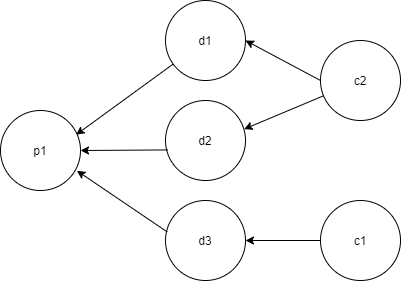
\includegraphics[scale=0.8]{figures/attack_relations.png}
    \caption{attack relations}
    \label{fig:attack relations}
\end{figure}

\subsubsection{Structuring Arguments in Argumentation Framework}

Let $AF$ be an Argumentation Framework \cite{dung1995} such that $AF$ = $<AR, attacks>$, 
where $AR$ is a set of arguments such that $AR = \{p_1, d_1, d_2, d_3, c_1, c_2\}$ and $attacks$ is a set of attack relations where $attacks$ = $\{(d_1, p_1), (d_2, p_1), (d_3, p_1), (c_1, d_1), (c_1, d_2), (c_2, d_3)\}$.

From this, it is easy to see that the admissable sets = $\{\{c_1\}, \{c_2\}, \{p_1, c_1\}, \{p_1, c_2\}, \{c_1, c_2\} \{p_1, c_1, c_2\}\}$, preferred extensions = $\{\{p_1, c_1, c_2\}\}$ and Grounded extensions = $\{p_1, c_1, c_2\}$

We can then find the interpretations of rules from the winning arguments by taking the union of the rules being applied in $p_1, c_1$ and $ c_2$.

i.e.

     Conditions to be applied to war risk coverage :-
    \begin{enumerate}
        \item proximate cause of loss is damage to ship due to a war risk.
        \item proximate cause does not fall under exemptions
    \end{enumerate}
    
     Proximate cause of loss :-
     
     \begin{enumerate}
        \item Ship is damaged due to rebel forces occupying ship firing at american forces.
        \item OR Ship is damaged due to american forces returning fire at rebels on the ship.
     \end{enumerate}
     
     conditions to NOT construe requisition in favour of defendant by Contra proferentem canon:
         \begin{enumerate}
             \item requisition is ambiguous.
             \item AND contract is written by defendant.
         \end{enumerate}


\FloatBarrier
